\documentclass[12pt]{scrartcl}
\usepackage[dutch]{babel}
\usepackage{CJK}
\usepackage[CJK, overlap]{ruby}
\usepackage{float}
\usepackage{graphicx}
\usepackage{multirow}

\renewcommand{\rubysep}{-0.2ex}


\begin{document}

%\begin{CJK*}[dnp]{JIS}{min}
\begin{CJK*}{UTF8}{min}
\CJKtilde
%\CJKcaption{JIS}

%
% Title page
%
\title{Aikibudo Terminologie}
\author{Andy Nagels}
\maketitle
\thispagestyle{empty} %should remove the page number
%\pagestyle{empty} %should remove the page number in the whole document
\begin{figure}[H]
\centering
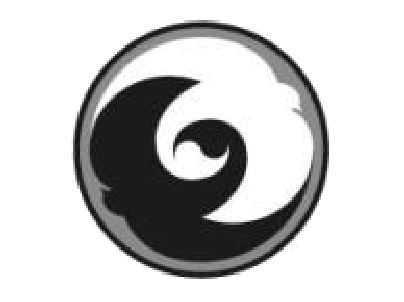
\includegraphics[width=2.5cm]{img/schild_aikibudo.eps}
\end{figure}

\begin{center}
合気武道
\end{center}

\begin{figure}[H]
\centering
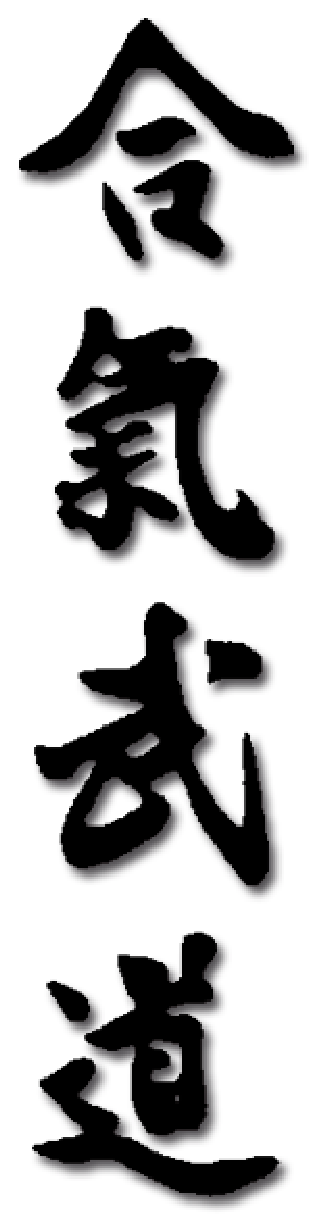
\includegraphics[width=1.0cm]{img/aikibudo-kanji.eps}
\end{figure}

%
% Disclaimer
%
\newpage
\begin{center}
\textbf{Disclaimer}\\
De vertalingen in dit document zijn gemaakt door mezelf, m.b.v. offici\"{e}le documenten, moderne technologie en mijn eigen kennis van het Japans. Daar ik echter geen expert ben in de Japanse taal, is het mogelijk dat er fouten staan in dit document. Naarmate mijn kennis van Aikibudo en Japans stijgt, zal ik de nieuwe kennis die ik heb opgedaan dan ook gebruiken om dit document na te kijken en te corrigeren.\\
Dit document is dus niet als finaal te beschouwen. Het wordt reeds vrijgegeven omdat het kan helpen bij het onthouden van de technieken.
\end{center}
\begin{center}
\textit{{\em Opmerking:} De laatste versie kan gratis gedownload worden van de volgende url: http://c.dommel.be/aikibudo.html.\\
Hier staat steeds de datum van laatste wijziging naast het document.}
\end{center}

%
% Table of contents
%
\newpage
\setcounter{page}{1}
\pagenumbering{Roman}
\tableofcontents

%
% Main content
%
\newpage
\setcounter{page}{1}
\pagenumbering{arabic}

% standard it's wadalab mincho, which gives the best results
%\CJKfamily{gothic}
\section{Inleiding}
\noindent Dit document bevat termen die gebruikt worden in aikibudo.

\section{De Japanse taal}
\noindent Alvorens we de berippen bekijken, dient een korte uitleg gegeven te worden over de Japanse taal.\\

\noindent Japans is opgebouwd uit 3 grote onderdelen: \textit{hiragana, katakana} en \textit{kanji}.\\

\noindent Hiragana en katakana zijn allebei een \textit{phonetisch} alfabet. Dat wil zeggen dat het symbolen voorstelt, die een klank uitbeelden.
Japans heeft dus geen aparte letters, zoals de meeste Westerse alfabetten.\\

\noindent \textbf{Hiragana} wordt gebruikt om zinnen te vormen en grammatica toe te passen op de Japanse taal. Het toont hoe Japans wordt uitgesproken.\\

\noindent \textbf{Katakana} bevat dezelfde klanken en enkele extra klanken. Het is ontstaan om de verschillende buitenlandse termen te kunnen uitspreken. Zo worden bvb. namen van niet Japanners in katakana geschreven.\\

\noindent \textbf{Kanji} zijn de meer complexe Japanse symbolen, die woorden en begrippen voorstellen. Ook Japanse namen en plaatsnamen worden meestal met kanji geschreven. Om te weten hoe deze symbolen worden uitgesproken, wordt gebruik gemaakt van hiragana, omdat hiragana een phonetisch alfabet is dat klanken in beeld brengt.\\

\noindent \textbf{Romaji} is een westerse schrijfwijze van Japanse klanken. Het wordt in Japan ook gebruikt om op een computer te typen.
Het is deze schrijfwijze, die het mogelijk maakt voor mensen die geen Japans kennen, om Japanse termen correct uit te spreken.

\noindent In de tabel hieronder, kan je een overzicht vinden van de verschillende alfabetten, ter verduidelijking van bovenstaande uitleg.\\

\begin{table}[H]
\begin{center}
\begin{tabular}{c|c|c|c}
Nederlands alfabet & Hiragana & Katakana & Romaji\\
\hline
a &  あ & ア & a\\
k & bestaat niet & bestaat niet & bestaat niet\\
bestaat niet & か & カ & ka
\end{tabular}
\end{center}
\caption{Een kleine vergelijking ter verduidelijking}
\label{vergelijking_alfabetten}
\end{table}

\noindent De begrippen in dit document, zijn op volgende manier weergegeven:\\

\textit{Nederlandse omschrijving} $|$ \textit{Japanse term [hiragana uitspraak]} $|$ \textit{romaji uitspraak}\\

\noindent De technieken zijn echter te lang om op die manier weer te geven. Zij staan dus onder elkaar:\\

\begin{center}
\textit{Nederlandse term}\\
\textit{Japanse term [hiragana uitspraak]}\\
\textit{Romaji uitspraak}
\end{center}

\section{Uitspraak}
\noindent Een aantal letters worden iets anders uitgesproken in de romaji uitspraak, t.o.v. het Nederlands.
Het is interessant om dit even te lezen, om zo geen verkeerde uitspraak te leren voor de techniek.\\

\noindent j: $|zj|$ zoals in strand\textbf{j}anet, \textbf{J}efke, ... (en NIET zoals in \textbf{J}ommeke)\\
ch: $|tsj|$ zoals in \textbf{tsj}oeke \textbf{tsj}oeke tuut tuut\\
sh: $|sj|$ zoals in \textbf{ch}oco, \textbf{sh}ampoo, ...\\
u: korte $|oe|$ zoals in nen t\textbf{oe}k \textbf{oe}p aa bakkes, vake en m\textbf{oe}ke, ...\\
\={o} of ou: lange $|o|$ zoals in b\textbf{oo}t\\
\={u} of uu: lange $|u|$ zoals in v\textbf{uu}r

\section{Algemene terminologie}
\subsection{Algemeen}
\begin{table}[H]
\begin{center}
\begin{tabular}{c|c|c}
basis/oorsprong/standaard & 基本 [きほん] & kihon \\
\hline
de kunst van het veilig vallen & 受身 [うけみ] & ukemi \\
\hline
actieve partner & 取り[どり] & dori\\
\hline
controle & 押さえ [おさえ] & osae\\
\hline
techniek & 技 [わざ] & waza\\
\hline
houding & 構え [かまえ] & kamae 
\end{tabular}
\end{center}
\end{table}

\subsection{Richtingen en gebieden}
\begin{table}[H]
\begin{center}
\begin{tabular}{c|c|c}
rechts & 右 [みぎ] & migi \\
\hline
links & 左 [ひだり] & hidari\\
\hline
achterwaarts & 後ろ[うしろ] & ushiro\\
\hline
voorwaarts & 前 [まえ] & mae\\
\hline
bovenste graad & 上段 [じょうだん] & j\={o}dan\\
\hline
midden & 中段 [ちゅうだん] & ch\={u}dan\\
\hline
grond & 土[ど] & do
\end{tabular}
\end{center}
\end{table}

\subsection{Acties}
\begin{table}[H]
\begin{center}
\begin{tabular}{c|c|c}
worp & 投げ [なげ] & nage\\
\hline
kopstoot & 頭突き [ずつき] & zutsuki\\
\hline
trap & 蹴り [けり] & keri\\
\hline
wurging & 絞殺 [こうさつ] & k\={o}satsu\\
\hline
omkering/terug sturen & 返し [がえし] & gaeshi\\
\hline
zijwaartse trap & 横蹴り [よこけり] & yoko keri\\
\hline
stoot & 突き [つき] & tsuki
\end{tabular}
\end{center}
\end{table}

\subsection{Lichaamsdelen}
\begin{table}[H]
\begin{center}
\begin{tabular}{c|c|c}
lichaam & 体 [たい] & tai \\
\hline
hand & 手[て] & te \\
\hline
elleboog/elleboogstoot & 肘 [ひじ] & hiji\\
\hline
knie & 膝 [ひざ] & hiza\\
\hline
pols & 手首 [てくび] & tekubi\\
\hline
onderarm & 小手 [こて] & kote\\
\hline
schouder & 肩 [かた] & kata
\end{tabular}
\end{center}
\end{table}

\subsection{Andere begrippen}
\begin{table}[H]
\begin{center}
\begin{tabular}{c|c|c}
schroef/veer van horloge & 捻子 [ねじ] & neji\\
\hline
uitwendig & 表 [おもて] & omote\\
\hline
tabel & 表 [ひょう] & hy\={o}
\end{tabular}
\end{center}
\end{table}

\subsection{Leerstof}
\begin{table}[H]
\begin{center}
\begin{tabular}{c|c|c}
verwijdering van het lichaam & 体捌き [たいさばき] & tai sabaki\\
\hline
valtechnieken & 受身技 [うけみわざ] & ukemi waza\\
\hline
stoottechnieken & 突き技 [つきわざ] & tsuki waza\\
\hline
traptechnieken & 蹴り技 [けりわざ] & keri waza\\
\hline
? & ? [ほじょうんど] & hojo undo\\
\hline
vrij gevecht & 乱取り [らんどり] & randori
\end{tabular}
\end{center}
\end{table}

\newpage
\section{級の技 Ky\={u} technieken}
\subsection{6de ky\={u} [SHOKU]}
\begin{table}[H]
\begin{center}
\begin{tabular}{c|c}
\textbf{verwijdering van het lichaam} & ?\\
\textbf{体捌き [たいさばき]} & ? [いりみ]\\
\textbf{tai sabaki} & irimi\\
\cline{2-2}
& ?\\
& ? [おいりみ]\\
& o irimi\\
\hline
\textbf{valtechnieken} & achterwaarts\\
\textbf{受身技 [うけみわざ]} & 後ろ [うしろ]\\
\textbf{ukemi waza} & ushiro\\
\hline
\textbf{stoottechnieken} & ?\\
\textbf{突き技 [つきわざ]} & ?\\
\textbf{tsuki waza} & ? \\
\hline
\end{tabular}
\end{center}
\label{kyuu_6}
\end{table}

\newpage
\subsection{5de ky\={u} [SHOKU]}
\subsubsection{Algemeen}
\subsubsection{技 Technieken}

\newpage
\subsection{4de ky\={u} [CHUKYU]}
\subsubsection{Algemeen}
\subsubsection{技 Technieken}

\newpage
\subsection{3de ky\={u} [CHUKYU]}
\subsubsection{Algemeen}
\subsubsection{技 Technieken}

\newpage
\subsection{2de ky\={u} [JOKYU]}
\subsubsection{Algemeen}
\subsubsection{技 Technieken}

\newpage
\subsection{1ste ky\={u} [JOKYU]}
\subsubsection{Algemeen}
\subsubsection{技 Technieken}

\newpage
\section{段の技 Dan technieken}
\subsection{第一段 1ste dan}
\subsubsection{Algemeen}
\begin{table}[H]
\begin{center}
\begin{tabular}{c}
zwarte gordel/persoon die een rang heeft\\
有段者[ゆうだんしゃ]\\
y\={u}dansha\\
\hline
1ste dan\\
第一段[だいいちだん]\\
daiichi dan
\end{tabular}
\end{center}
\label{dan_1_gen}
\end{table}

\subsubsection{技 Technieken}
\begin{table}[H]
\begin{center}
\begin{tabular}{c}
?\\
? [ひらき]\\
hiraki\\
\hline
weegschaal worp\\
天秤投げ [てんびんあげ]\\
tenbin nage\\
\hline
veer/schroef van horloge onderarm omkering\\
螺子小手返し [ねじこてがえし]\\
neji kote gaeshi\\
\hline
?\\
螺子小手返し [ねじこてがえし]\\
\end{tabular}
\end{center}
\label{dan_1}
\end{table}

\newpage
\subsection{2de dan}
\subsubsection{Algemeen}
\begin{table}[H]
\begin{center}
\begin{tabular}{c}
2de dan\\
第二段[だいにだん]\\
daini dan
\end{tabular}
\end{center}
\label{dan_2_gen}
\end{table}

\subsubsection{技 Technieken}

\newpage
\subsection{3de dan}
\subsubsection{Algemeen}
\begin{table}[H]
\begin{center}
\begin{tabular}{c}
3de dan\\
第三段[だいさんだん]\\
daisan dan
\end{tabular}
\end{center}
\label{dan_2_gen}
\end{table}

\subsubsection{技 Technieken}

\newpage
\section{表技 Omote waza}
\subsection{基本投げ技 Kihon nage waza (7 technieken)}

\subsection{基本押え技 Kihon osae waza (6 technieken)}

\subsection{雄用技投げ技 Oy\={o} waza nage waza (間 - 近間)}
\begin{table}[H]
\begin{center}
\begin{tabular}{c}
technieken voor mannen werp technieken(ruimte laten - dichtbij)\\
雄用技投げ技(間 - 近間)\\
oy\={o} waza nage waza (ma - chikama)\\
\end{tabular}
\end{center}
\label{oyouwazanagewaza}
\end{table}

\subsection{雄用技押え技 Oy\={o} waza osae waza [間 - 近間]}
\begin{table}[H]
\begin{center}
\begin{tabular}{c}
technieken voor mannen werp technieken(ruimte laten - dichtbij)\\
雄用技押え技(間 - 近間)\\
oy\={o} waza osae waza (ma - chikama)\\
\end{tabular}
\end{center}
\label{oyouwazaosaewaza}
\end{table}

\subsection{和の精神 Wa no sei shin}
\begin{table}[H]
\begin{center}
\begin{tabular}{c}
geest in harmonie\\
和の精神[わのせいしん]\\
wa no sei shin\\
\hline
voorwaarts en achterwaarts - lijn van het lichaam\\
前 と 後 - 体の線\\
mae to ushiro - tai no sen
\end{tabular}
\end{center}
\label{wanoseishin}
\end{table}

\subsection{乱取り Randori}
\begin{table}[H]
\begin{center}
\begin{tabular}{c}
vrij gevecht\\
乱取り[らんどり]\\
randori\\
\hline
zacht gevecht (ruimte laten - lijn van het lichaam)\\
柔の乱取り (間 - 体の線)[じゅうのらんどり (ま - たいのせん)] \\
j\={u} no randori (ma - tai no sen)
\end{tabular}
\end{center}
\label{randori}
\end{table}

\subsection{形大東流 - ? Kata dait\={o} ry\={u} - ikajo}

\newpage
\section{Tenshin Sh\={o}den Katori Shint\={o} Ry\={u}}
\subsection{Algemeen}
\begin{table}[H]
\begin{center}
\begin{tabular}{c}
de weg van de hemel gewijdt aan de positieve legende van het Katori altaar\\ 
天真正傳香取神道流[てんしんしょうでんかとりしんとうりゅう]\\
tenshin sh\={o}den katori shint\={o} ry\={u}
\end{tabular}
\end{center}
\label{katori}
\end{table}


\subsection{6de ky\={u}}
\subsubsection{構え kamae}
\begin{table}[H]
\begin{center}
\begin{tabular}{c}
bovenste/hoge houding\\
上段の構え[じょうだんのかまえ]\\
j\={o}dan no kamae\\
\hline
houding met de katana gericht naar de ogen van de tegenstander\\
青眼の構え[せいがんのかまえ]\\
seigan no kamae\\
\hline
boog onder een hoek\\
弧がすみ[こがすみ]\\
ko gasumi\\
\hline
hand naar achteren onder een hoek\\
手裏がすみ[てうらあがすみ]\\
te ura gasumi\\
\hline
rechter lagere houding\\
右下段の構え[みぎげだんのかまえ]\\
migi gedan no kamae\\
\hline
linker lagere houding (omgekeerde lagere)\\
左下段の構え[ひだりげだんおかまえ]\\
hidari gedan no kamae (gyaku gedan)\\
\hline
schaduw houding\\
陰の構え[いんのかまえ]\\
in no kamae\\
\hline
schuine houding\\
斜の構え[しゃのかまえ]\\
sha no kamae\\
\hline
rechter hoge houding\\
右上段の構え[みぎじょうだんのかまえ]\\
migi j\={o}dan no kamae\\
\hline
linker hoge houding\\
左上段の構え[ひだりじょうだんのかまえ]\\
hidari j\={o}dan no kamae\\
\hline
? houding\\
? [しんのかまえ]\\
shin no kamae\\
\hline
? onder een hoek\\
? [おがすみ]\\
o gasumi\\
\hline
lager zitten (in houding)\\
座り下段(の構え)[すわりげだんのかまえ]\\
suwari gedan (no kamae)\\
\hline
vogelstand\\
鳥[とり]\\
tori
\end{tabular}
\end{center}
\label{kyuu_6_katori_kamae}
\end{table}

\subsubsection{技 Technieken}
\noindent Alleen en in kumitachi.
\begin{table}[H]
\begin{center}
\begin{tabular}{c}
uitrol van een winding\\
巻き打ち[まきうち]\\
maki uchi\\
\hline
uitrol zijkant van het gezicht\\
横面打ち[よこめんうち]\\
yokomen uchi\\
\hline
uitrol naar de grond (volledige snijbeweging van boven naar onder)\\
土打ち[どうち]\\
do uchi\\
\hline
bodem ontvangen\\
土受け[どうけ]\\
do uke\\
\hline
punt katana laten zakken en katana wegsteken\\
?[?]\\
noto
\end{tabular}
\end{center}
\label{kyuu_6_katori_other}
\end{table}

\subsection{5de ky\={u}}
\subsubsection{kata}
\begin{table}[H]
\begin{center}
\begin{tabular}{c}
?\\
?\\
ken no kata\\
\hline
?\\
?\\
bo no kata\\
\hline
?\\
?\\
kusanagi no ken (iai goshi)
\end{tabular}
\end{center}
\label{kyuu_5_katori_kata}
\end{table}

\subsubsection{bo jutsu}
\noindent Alleen en in kumitachi.
\begin{table}[H]
\begin{center}
\begin{tabular}{c}
?\\
?\\
yokomen uchi\\
\hline
?\\
?\\
do uchi\\
\hline
?\\
?\\
sune uchi
\end{tabular}
\end{center}
\label{kyuu_5_katori_bo}
\end{table}

\subsection{4de ky\={u}}
\subsubsection{kata}
\begin{table}[H]
\begin{center}
\begin{tabular}{c}
?\\
?\\
itsutsu no tachi (kiri komi)\\
\hline
?\\
?\\
nuki tsuke no ken (iai goshi)
\end{tabular}
\end{center}
\label{kyuu_4_katori_kata}
\end{table}

\subsection{3de ky\={u}}
\subsubsection{kata}
\begin{table}[H]
\begin{center}
\begin{tabular}{c}
?\\
?\\
nanatsu no tachi (kiri komi)\\
\hline
?\\
?\\
nuki uchi no ken (iai goshi)\\
\hline
?\\
?\\
seri ai no bo (uchi komi)
\end{tabular}
\end{center}
\label{kyuu_3_katori_kata}
\end{table}

\subsection{2de ky\={u}}
\subsubsection{kata}
\begin{table}[H]
\begin{center}
\begin{tabular}{c}
?\\
?\\
kasumi no tachi (kiri komi)\\
\hline
?\\
?\\
sune hishigi no bo (uchi komi)\\
\hline
?\\
?\\
itsutsu no naginata (kiri komi)\\
\hline
?\\
?\\
uken (iai goshi)
\end{tabular}
\end{center}
\label{kyuu_2_katori_kata}
\end{table}

\subsection{1ste ky\={u}}
\subsubsection{kata}
\begin{table}[H]
\begin{center}
\begin{tabular}{c}
?\\
?\\
haka no tachi (kiri komi)\\
\hline
?\\
?\\
saken (iai goshi)\\
\hline
?\\
?\\
happo ken (iai goshi)
\end{tabular}
\end{center}
\label{kyuu_1_katori_kata}
\end{table}

\subsection{第一段 1ste dan}
\subsubsection{kata}
\noindent Een perfecte kennis is vereist van alle voorgaande technieken.\\

\subsubsection{extra}
\begin{itemize}
\item Houding van het lichaam en perfectie van de posities: shisei
\item Uitgesproken expressie van kime, zanshin en kiai
\item Kennis van de kobudo termen en de verschillende onderdelen waaruit een katana is opgebouwd
\end{itemize}

\end{CJK*}
\end{document}
